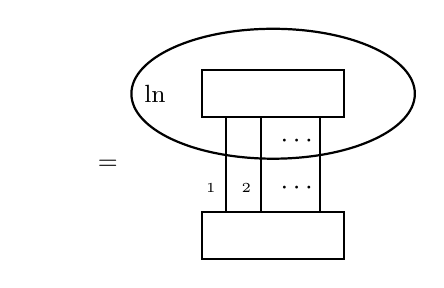
\begin{tikzpicture}[scale=0.3,thick] % , baseline = -3.5pt

\node[anchor=center] (text) at (-8,-5) {\small $\sentropyof{\probtensor}$};

\node[anchor=center] (text) at (-5,-5) {\small ${=}$};

\node[anchor=center] (text) at (-3,-2) {\small $\mathrm{ln}$};
\draw (2,-2) ellipse (6 and 2.75);

\draw (-1,-1) rectangle (5,-3);
\node[anchor=center] (text) at (2,-2) {\small $\probtensor$};
\draw (-1,-7) rectangle (5,-9);
\node[anchor=center] (text) at (2,-8) {\small $\probtensor$};
\draw (0,-5)--(0,-3); 
\draw (0,-5)--(0,-7) node[midway,left] {\tiny $\atomlegindexof{1}$}; 
\draw (1.5,-5)--(1.5,-3); 
\draw (1.5,-5)--(1.5,-7) node[midway,left] {\tiny $\atomlegindexof{2}$}; 
\node[anchor=center] (text) at (3,-4) {$\cdots$};
\draw (4,-5)--(4,-3);
\node[anchor=center] (text) at (3,-6) {$\cdots$};
\draw (4,-5)--(4,-7) node[midway,right] {\tiny $\atomlegindexof{\atomorder}$}; 

%\drawatomcore{3.5}{-8}{$\probtensor$}
%\drawatomindices{3.5}{-12}	
%\draw (5.5,-9)--(5.5,-7) node[midway,right] {\tiny $\atomlegindexof{\exformula}$};

\end{tikzpicture}